\section{Benchmarks}
To measure the perfomance of our Advert service solution, we performed
benchmarks on our Google App Engine Advert Service library. We executed a
couple of tests to measure latency, bandwidth, and server-side performance.
Below we describe our benchmarks in more detail.

All measurements below were perfomed on a 2.16 GHz Intel Core 2 Duo iMac, with
1GB 667 MHz DDR2 SDRAM (unless stated otherwise). Network performance may vary,
depending on your bandwidth and network traffic. We did our measurements from
the \emph{Vrije Universiteit}, which owns a fibreglass internet connection
provided by \emph{SURFnet} (unless stated otherwise).

Furthermore, we used the UNIX \texttt{traceroute} command to determine where our
App Engine application is hosted. The results can be found in figure
\ref{tracert}. The last known IP address resides at Mountain View, California
(US), which is where Google Inc. is residing. It is safe to assume that all our
request go to Google US and back.

\begin{figure*}[ht] %[placement] where placement is h,t,b,p
\begin{center}
\begin{code}
$ traceroute ibisadvert.appspot.com
traceroute to appspot.l.google.com (74.125.79.141), 64 hops max, 40 byte packets
 1  router-student1 (130.37.24.7)  0.641 ms  0.314 ms  0.293 ms
 2  hkae16-2-d02.backbone.vu.nl (130.37.5.54)  0.288 ms  0.257 ms  0.274 ms
 3  GE5-1-1.2090.JNR01.Asd002A.surf.net (145.145.20.57)  0.674 ms  0.665 ms  0.620 ms
 4  AE0.500.JNR02.Asd002A.surf.net (145.145.80.65)  0.690 ms  0.657 ms  0.745 ms
 5  core1.ams.net.google.com (195.69.144.247)  1.156 ms  0.993 ms  0.997 ms
 6  209.85.248.93  11.159 ms  1.353 ms  1.269 ms
 7  64.233.175.246  14.791 ms 72.14.233.114  6.209 ms 64.233.175.246  4.269 ms 
 8  72.14.239.199  5.749 ms 209.85.255.166  5.932 ms 72.14.239.197  4.606 ms 
 9  209.85.255.126  7.864 ms 209.85.255.122  6.025 ms  6.676 ms 
 10  * * *
\end{code}
\caption{Traceroute output of ibisadvert.appspot.com.\label{tracert}}
\end{center}
\end{figure*}

\subsection{Initialization}
Initializing our Advert library can be done in two different ways. First, we
have the public Advert server, which does not require any authentication 
whatsoever. Initializing this class takes a negligible amount of time (i.e.
less than 0ms).

Secondly, we have a private server model, which does require authentication.
Authenticating to a private Advert server can be divided in three parts:

\begin{itemize}
  \item Authenticating to Google using ClientLogin
  \item Retrieving a authentication cookie from the Google App Engine
  \item Initializing and starting up `Persistent Authentication' thread
\end{itemize}

We measured the total time of initializing the Advert library (client-side),
which has an average of 190ms (179ms minimum, 229ms maximum). In addition we
measured each of the parts above individually, after which we can conclude that
authenticating using ClientLogin takes up one-third of the latency stated above,
and retriving the authentication cookie takes up two-third of the time measured
above. Initializing and starting up our `Persistent Authentication' thread
takes a negligible amount of time (i.e. less than 0ms).

Note that it is impossible to measure server-side performance/latency, because
ClientLogin and the process of retrieving a authentication cookie from the
Google App Engine, are both closed source procedures at Google, in which we
cannot place any timers.

As from now, all measurements will be done with respect to the authenticated
server, because we expect it will be used most in practice.

\subsection{Client Functions}
Another interesting thing to measure is the latency generated by various client
functions, and how this latency increases when we process greater amounts data.
We conducted measurements of calling all client functions with variable amounts
of data. Results can be viewed below:

\subsubsection{Add}
The process of adding an object to the datastore consists of four parts.

\begin{itemize}
  \item Processing the object (encoding to Base64 and JSON) and meta data
  \item Sending the object to the advert server
  \item Storing (possibly overwriting) the object and meta data
  \item Receiving a response
\end{itemize}

Notably, latency will increase as data-to-process increases. That's why we
conducted measurements with a variable object and meta data size. Note that
Google's datastore API has a maximum call size of 1MB, and since we are
encoding all our objects in Base64, the objects to add should be roughly 1.4
times smaller than what we really want to store. Therefore, we stored objects 
of size 730Bytes, 7.300Bytes, 73.000Bytes, and 730.000Bytes (being 1kB, 10kB,
100kB, and 1.000kB of data stored, respectively).

\paragraph{Variable Object Size}
Below we state the results of the measurements we did client-side. Note that
the client-side measurements are network latency dependent, where the
server-side measurements are not (see Figure \ref{add-obj-size}). We added an
object (without meta data), of variable size, to the datastore ten times.

If we look at the subdivision of adding an object to the datastore, client
side, we see that for all results that encoding the data to Base64 takes a
negligible amount of time (less than 1\% of the total time, except when we add
730.000Bytes, this takes 2.6\% of the total time). 

\begin{figure}[ht] %[placement] where placement is h,t,b,p
\begin{center}
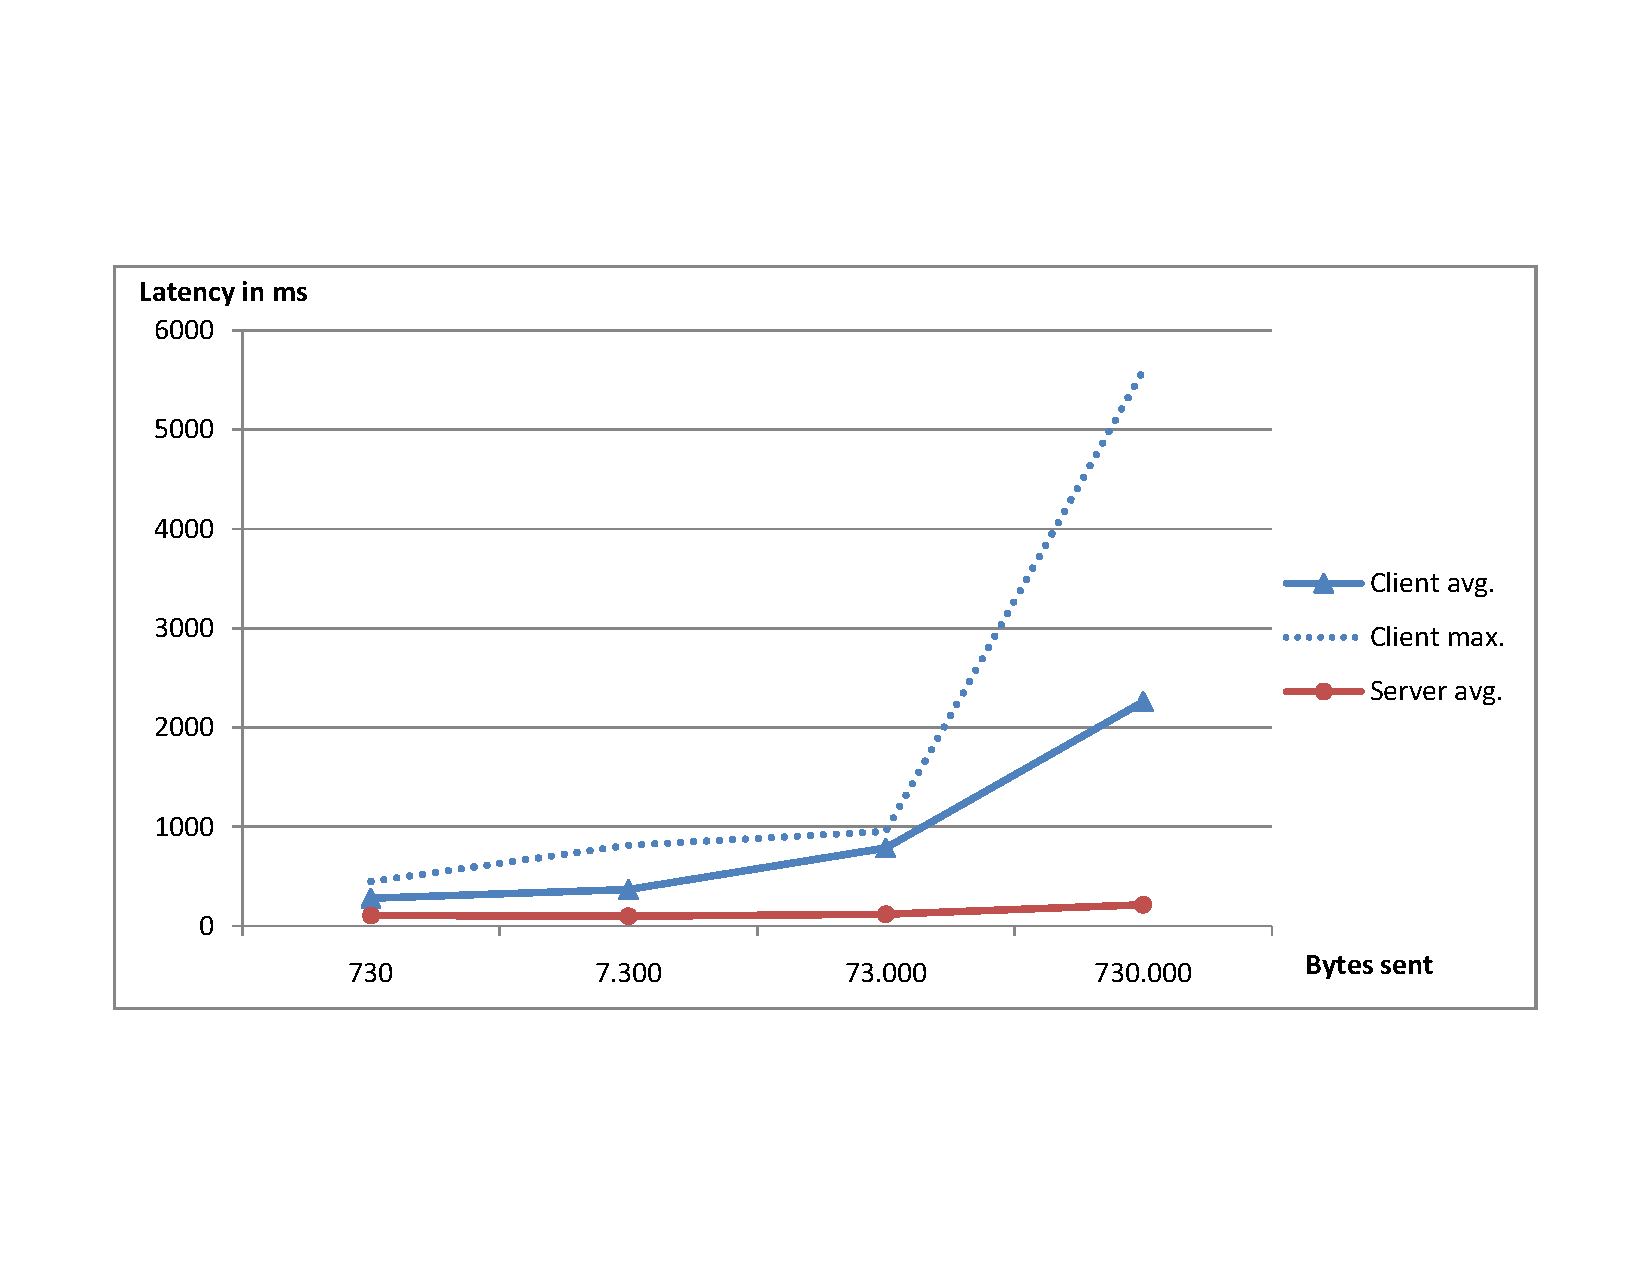
\includegraphics[trim=5cm 4cm 5cm 5cm,width=10cm]{add_obj.pdf}
\caption{Adding Objects of Variable Size. \label{add-obj-size}}
\end{center}
\end{figure}

\paragraph{Variable Meta Data Size}
In addition to varying object sizes, we also added an object (of size 730Bytes)
to the datastore, with a variable number of key-value pairs. We chose sending 0
pairs, 5 pairs, 25 pairs, 50 pairs, and 100 pairs. For results, see figure
\ref{add-md-size}.

Also the time to convert a \texttt{MetaData} object to JSON takes a negligible
amount of time (less than 1\% of the total time), even when adding large numbers
of key-value pairs (e.g. 100 pairs).

\begin{figure}[ht] %[placement] where placement is h,t,b,p
\begin{center}
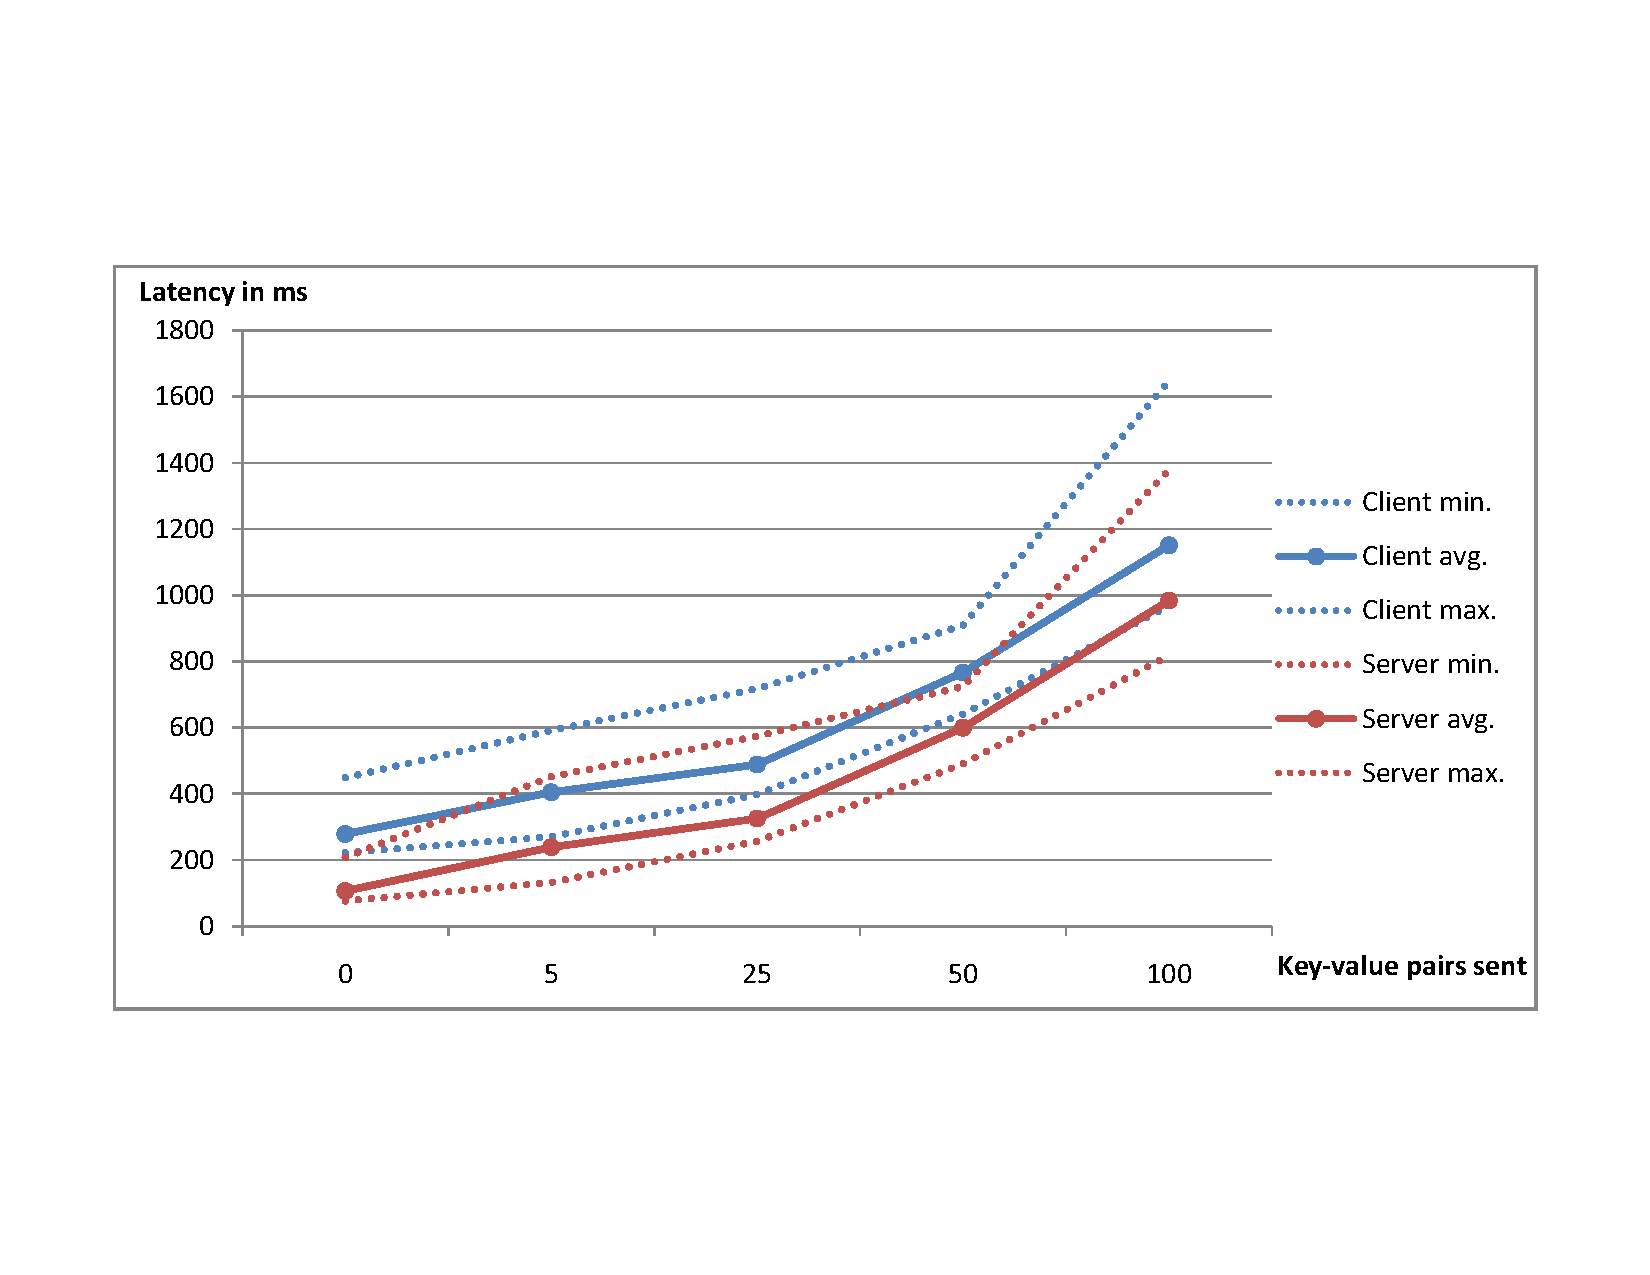
\includegraphics[trim=5cm 4cm 5cm 5cm,width=10cm]{add_md.pdf}
\caption{Adding Objects with Variable Meta Data. \label{add-obj-size}}
\end{center}
\end{figure}

\paragraph{Overwrite}
Note that two occasions can occur server-side: an entry does not exist yet; the
object is stored in the datstore. An object does already exits; the object is
overwritten. We tested the latency at the server side by sending a various
number of bytes, with and without any meta data to see how the latency
increases. Ideally the maximum latency wouldn't exceed the sum of the latencies
of a \texttt{del()} and an \texttt{add()} statement (that's what overwrite
does locally).

\begin{figure}
\begin{tabular}{|l|r|r|r|}
\hline
 & Min. & Avg. & Max. \\
\hline
No Overwrite & 173ms & 213ms & 292ms \\
Overwrite & 355ms & 425ms & 552ms \\
\hline
\end{tabular}
\caption{Server}
\end{figure}

\subsubsection{Get}
After an element is stored in the datastore, it can be retrieved by a client.
In this case, we tested the 10 elements residing in the datstore, all of the
same size. Next, we retrieved every element from the datastore sequentially and
measured the time to do so client and server-side (see Figure
\ref{get-obj-size}). Note that we will not vary the number of Meta Data items,
because those are not fetched using the \texttt{get()} function.

As for client-side measurements. Decoding from Base64 to the actual binary
object takes a negligible amount of time (less than or equal to 1ms).

Finally, we will see if latency increases (server-side), if the number of
entries in the datatore increase. We measured server-side latency with a
varialbe number of entries in the datastore (10, 100, 1000), where all objects
are the same size (for results, see Figure \ref{get-obj-amt}). According to
Google, the latency should stay consistent, and as we can see from Figure
\ref{get-obj-amt}, its average stays around 25 to 30ms.

% \begin{figure}
% \begin{tabular}{|r|r|r|r|}
% \hline
% Bytes received & Min. & Avg. & Max. \\
% \hline
% \multicolumn{4}{|c|}{Client side} \\
% \hline
% 730 & 151ms & 162ms & 176ms \\
% 7.300 & 165ms & 186ms & 274ms \\
% 73.000 & 213ms & 249ms & 403ms \\
% 730.000 & 452ms & 537ms & 766ms \\
% \hline
% \multicolumn{4}{|c|}{Server side} \\
% \hline
% 730 & 27ms & 30ms & 34ms \\
% 7.300 &  \\
% 73.000 &  \\
% 730.000 &  \\
% \hline
% \end{tabular}
% \caption{Receiving Different Object Sizes. \label{get-obj-size}}
% \end{figure}

% \begin{figure}
% \begin{tabular}{|r|r|r|r|}
% \hline
% \# Entries in datastore & Min. & Avg. & Max. \\
% \hline
% \multicolumn{4}{|c|}{Server side} \\
% \hline
% 10 & 27ms & 30ms & 34ms \\
% 100 & 22ms & 26ms & 30ms \\
% 1000 & 23ms & 30ms & 36ms \\
% \hline
% \end{tabular}
% \caption{Receiving Objects With Different Amounts in Datastore.
% \label{get-obj-amt}}
% \end{figure}

\subsubsection{Delete}
Deleting an item from the datastore should not be an issue at the client side
(the client sends the pathname of the object to be deleted, and \texttt{OK} or
\texttt{Not Found} is returned accordingly). Hence, we only measured the
\texttt{delete()} function at the server side. 

Again, we are curious to see if the server needs more time to delete an item
when the datastore is full of data or almost empty (it should not make any
difference, since the functionality is much alike the \texttt{get()} function).
Similar to \texttt{get()}, we timed the \texttt{delete()} statement for a
varialbe number of entries in the datastore (10, 100, 1000), where all objects
are the same size (for results, see Figure \ref{del-obj-amt}).

% \begin{figure}
% \begin{tabular}{|r|r|r|r|}
% \hline
% \# Entries in datastore & Min. & Avg. & Max. \\
% \hline
% \multicolumn{4}{|c|}{Server side} \\
% \hline
% 10 & 79ms & 92ms & 104ms  \\
% 100 & 82ms & 89ms & 94ms \\
% 1000 & 80ms & 94ms & 129ms \\
% \hline
% \end{tabular}
% \caption{Deleting Objects With Different Amounts in Datastore.
% \label{del-obj-amt}}
% \end{figure}

\section{Bandwidth}
In addition to latency, we also tried to measure the bandwidth between the
Vrije Universiteit, Amsterdam, and the Google App Engine (located as stated in
Figure \ref{tracert}).

First of all, we measured the round-trip delay, by creating a dummy server
which would instantly reply the shortest possible message to the client. Also,
the client would only send a GET request and wait for a response code. We
measured the round-trip delay to be 120ms on average.

Next we measured the upload bandwidth (of the client), by sending the maximum
request size (10MB) to the server, and letting the server send an empty message
back as minimum response. We measured this to be 5113ms on average. 

Finally, we measured the download bandwidth (client-side), by doing a GET
request of 10MB. The server would actually have to read a 10MB file and return
it to the client. Reading this file also has a little overhead (approximately
130ms), so we substract that form our measured results, which gives us a
round-trip delay of 26387ms on average. Our download fluctuated quite a bit,
this might be the cause of multiple users using the same internet connection
for various purposes.

Finally, we want to know our bandwith in kB/sec. This we calculate by
substracting the round-trip delay from the upload and download round-trip
delays measured. Which gives us 4983ms and 26257ms respectively. Now, we divide
the number of bytes sent (10.000.000bytes each), by the number of seconds, and
divide it by 1024 to get the kB/sec. We can conclude that our upload bandwidth
is 1960kB/sec, and our download bandwidth is 372kB/sec. \textbf{TODO: ik denk
dat het downloaden ook slow kan gaan door de manier waarop Java de byte stream
uitleest.}



